% ============================================================
%  sec06b.tex —— §6.2 椭圆曲线的导出范畴 / §6.3 环面的 Fukaya 范畴
%  对应原文 pp.29–38（含无编号小节 Equivariant $A_\infty$-structures and
%  Weierstrass cubics、Generation、Counting polygons）
%  本文件不含 \section：§6 的 \section 与 §6.1 在 sec05_06a.tex 中。
% ============================================================

\subsection{椭圆曲线的导出范畴}\label{subsec:6.2}

固定一个特征零的代数闭域 $k$。令 $E$ 为光滑射影曲线，$P\in E$ 为闭点。由关于曲线导出范畴生成元的定理~\ref{thm:3.3}，$\mathcal{L}=\mathcal{O}_E\oplus\mathcal{O}_E(P)$ 是分裂生成元（split-generator）。由第~\ref{sec:derived} 节中 $D_\infty(E)$ 的构造、特别是命题~\ref{prop:3.1}，有
\[
\mathrm{Hom}_{HD_\infty(E)}(\mathcal{L},\mathcal{L})=\mathrm{Ext}^*(\mathcal{L},\mathcal{L}).
\]
这个分次代数的向量空间结构可以完全形式地确定；我们先做这一步。

% [Tutor Note: 易错点：Serre 对偶 $H^k(X,\mathcal{L})\cong H^{n-k}(X,\mathcal{L}^{\vee}\otimes\omega_X)^{\vee}$ 右端的对偶取自整个向量空间，而非层的对偶。对椭圆曲线 $n=1$、$\omega_X\cong\mathcal{O}_X$ 平凡，故 $H^1(E,\mathcal{L})\cong H^0(E,\mathcal{L}^{\vee})^{\vee}$；这是本节所有 Ext 群计算（尤其 $h_0h_1\neq0$、$h_1h_0\neq0$）的唯一非形式输入。]

事实上，回忆概形上 Ext 群的一些基本性质（见文献 [8] 第 III.6 节）：(1) 若 $\mathcal{L}$ 局部自由而 $\mathcal{F},\mathcal{G}$ 凝聚，则 $\mathrm{Ext}^*(\mathcal{L}\otimes\mathcal{F},\mathcal{G})=\mathrm{Ext}^*(\mathcal{F},\mathcal{L}^{\vee}\otimes\mathcal{G})$；(2) $\mathrm{Ext}^*(\mathcal{O}_X,\mathcal{F})=H^*(X,\mathcal{F})$；(3) $\mathrm{Ext}^*$ 是双线性的。这里 $\mathcal{L}^{\vee}$ 表示对偶层。这三条都是关于 $\mathrm{Hom}=\mathrm{Ext}^0$ 的相应陈述与导出函子泛性的容易推论。再回忆 Serre 对偶（见文献 [8] 第 III.7 节）：若 $X$ 是 $n$ 维光滑射影概形，则
\[
H^k(X,\mathcal{L})\cong H^{n-k}(X,\mathcal{L}^{\vee}\otimes\omega_X)^{\vee}.
\]

现在回到 $X=E$、$\mathcal{L}=\mathcal{O}_E\oplus\mathcal{O}_E(P)$ 的情形。此后我们一并省略下标 $E$。利用双线性，可以把 Ext 代数分解为“矩阵元”：
\begin{equation}\label{eq:6.2-1}
\mathrm{Ext}^*(\mathcal{L},\mathcal{L})=
\begin{pmatrix}
\mathrm{Ext}^*(\mathcal{O},\mathcal{O}) & \mathrm{Ext}^*(\mathcal{O}(P),\mathcal{O})\\[2pt]
\mathrm{Ext}^*(\mathcal{O},\mathcal{O}(P)) & \mathrm{Ext}^*(\mathcal{O}(P),\mathcal{O}(P))
\end{pmatrix}.
\end{equation}
这句话的意思是：左端作为向量空间分解为右端四个子空间的直和，而左端的乘法对应右端的矩阵乘法，再复合上 $\mathrm{Ext}^*=\mathrm{Hom}_{HD_\infty(E)}$ 上的外乘法。此外，我们可以用性质 (1)、(2) 连同 Serre 对偶，把上式用层上同调空间表出。

% [Tutor Note: 易错点：这里的“矩阵乘法”指由两个直和因子诱导的分块乘法，交叉项 $h_0h_1$、$h_1h_0$ 的符号遵循 Koszul 约定（$h_1$ 是度为 1 的奇元素）；原文只关心非零性，故未写符号。又，原文此句把 $\mathrm{Ext}^*=\mathrm{Hom}_{HD_\infty(E)}$ 的变量省略了，应读作 $\mathrm{Ext}^*(\mathcal{L},\mathcal{L})=\mathrm{Hom}_{HD_\infty(E)}(\mathcal{L},\mathcal{L})$；译文保留原文省略写法。]

下面特殊化到椭圆曲线情形，得到：

\begin{proposition}\label{prop:6.3}
设 $E$ 是特征零代数闭域 $k$ 上的椭圆曲线，$P\in E$ 为闭点。则
\[
\mathrm{Ext}^*(\mathcal{O}\oplus\mathcal{O}(P),\mathcal{O}\oplus\mathcal{O}(P))\xrightarrow{\ \sim\ }Q,
\]
其中 $Q$ 是上一小节的分次代数。
\end{proposition}

\begin{proof}
绝大部分工作已经完成。我们有 $H^0(E,\mathcal{O})=k$（即 $E$ 上没有非常值正则函数，这对任何连通射影概形都成立），于是特别地 $H^0(E,\mathcal{O}(-P))=0$（因为 $\mathcal{O}(-P)$ 是在 $P$ 处取零的正则函数构成的层）。又 $H^0(E,\mathcal{O}(P))=k$，因为 $E$ 不可能具有只有一个单极点的有理函数（否则它就同构于 $\mathbb{P}^1$）。注意到椭圆曲线的典范丛平凡，这些计算已足以说明我们的 Ext 代数作为分次向量空间同构于 $Q$。

但 $A$ 中本质上所有合成都已由形式理由确定（即由 $\mathcal{O}$ 与 $\mathcal{O}(P)$ 的单位元的作用，以及次数理由）。令 $h_0$ 表示 $\mathrm{Hom}(\mathcal{O},\mathcal{O}(P))$ 中的非零元，$h_1$ 表示 $\mathrm{Ext}^1(\mathcal{O}(P),\mathcal{O})$ 中的非零元。为完成证明，只需说明 $h_0h_1\neq0$ 且 $h_1h_0\neq0$，因为这是仅剩的尚未确定的合成。

% [Tutor Note: 原文此处记号 $A$ 未加定义，从上下文看它就是本段所论的 Ext 代数 $\mathrm{Ext}^*(\mathcal{L},\mathcal{L})$（原文此处作斜体 $A$、而非花体 $\mathcal{A}$；按行文它也可能是想写 §6.1 的 $Q$，但 $Q$ 此时只被证明为分次向量空间同构，尚不能直接当作代数使用）。译文保留原文记号。]

我们有正合列 $0\to\mathcal{O}\to\mathcal{O}(P)\to\mathcal{O}/P\to0$，其中第一个映射是 $h_0$。作用 $\mathrm{Ext}^*(\mathcal{O}(P),\bullet)$ 得到
\[
\mathrm{Ext}^1(\mathcal{O}(P),\mathcal{O})\xrightarrow{\ \times h_0\ }\mathrm{Ext}^1(\mathcal{O}(P),\mathcal{O}(P))\to\mathrm{Ext}^1(\mathcal{O}(P),\mathcal{O}/P).
\]
但 $\mathrm{Ext}^1(\mathcal{O}(P),\mathcal{O}/P)=H^1(E,\mathcal{O}/P)$（因为 $\mathcal{O}/P$ 是摩天楼层），而该群为零（摩天楼层是松弛的，即 flasque）。因此右乘 $h_0$ 是满射，且 $h_1h_0\neq0$。

% [Tutor Note: 作者省略的两步：($i$) $\mathrm{Ext}^1(\mathcal{O}(P),\mathcal{O}/P)=H^1(E,\mathcal{O}/P)=0$ 的理由是 $\mathcal{O}/P$ 为摩天楼层，而松弛层无高次上同调；($ii$) 后文 $\mathrm{Ext}^2(\mathcal{O}/P,\mathcal{O})=0$ 由对 $0\to\mathcal{O}\to\mathcal{O}(P)\to\mathcal{O}/P\to0$ 作用 $\mathrm{Ext}^*(\mathcal{O},\bullet)$ 并利用 $H^2(X,\mathcal{F})=0$ 得到，而后者对线丛成立——对椭圆曲线这正是 Serre 对偶 $H^2\cong H^0(\mathcal{F}^{\vee})^{\vee}=0$。]

改作用 $\mathrm{Ext}^*(\bullet,\mathcal{O})$，则得到
\[
\mathrm{Ext}^1(\mathcal{O}(P),\mathcal{O})\xrightarrow{\ h_0\times\ }\mathrm{Ext}^1(\mathcal{O},\mathcal{O})\to\mathrm{Ext}^2(\mathcal{O}/P,\mathcal{O}).
\]
只要确立 $\mathrm{Ext}^2(\mathcal{O}/P,\mathcal{O})=0$，前面的论证就同样行得通。而这可由对我们的正合列作用 $\mathrm{Ext}^*(\mathcal{O},\bullet)$、并注意到对任意线丛 $\mathcal{F}$ 有 $H^2(X,\mathcal{F})=0$（由 Serre 对偶）得到。
\end{proof}

我们指出：若 $P$ 是光滑点，则上述结果对奇异三次曲线仍然成立，只是此时论证要稍微仔细一些。

\subsubsection{\texorpdfstring{等变 $A_\infty$-结构与 Weierstrass 三次曲线}{等变 A∞-结构与 Weierstrass 三次曲线}}\label{subsec:equivariant-ainf}

我们希望论证：由椭圆曲线得到的 $Q$ 上的 $A_\infty$-结构本质上穷尽了所有可能（有两个例外，一个形式、一个非形式）。

具体地说，固定一条三次曲线 $E$ 与一个光滑点 $P$，并置
\[
\mathcal{Q}_{E,P}=\mathrm{Hom}_{D_\infty(E)}(\mathcal{O}_E\oplus\mathcal{O}_E(P),\mathcal{O}_E\oplus\mathcal{O}_E(P)).
\]
这是一个 DGA（微分分次代数），在拟同构意义下良定义；由前面的命题~\ref{prop:6.3}，有 $H(\mathcal{Q}_{E,P})\xrightarrow{\sim}Q$。于是由同调微扰论，我们得到 $Q$ 上的极小 $A_\infty$-结构 $(m_d^{E,P})$。

我们希望说：这样一来就得到了所有同构类的 $A_\infty$-结构。这件事出人意料地棘手。我们沿用文献 [11] 的方法，即研究如何把所有的 $\mathcal{Q}_{E,P}$ 一致地变成极小 $A_\infty$-代数。

% [Tutor Note: 几何直观：$\mathcal{Q}_{E,P}$ 是“把曲线上的两个对象 $\mathcal{O}$ 与 $\mathcal{O}(P)$ 之间的全部 Ext 群堆成一个 dg 代数”；它依赖 $E,P$ 的选取，但只在拟同构意义下良定义。同调微扰论把它的极小模型搬到 $H(\mathcal{Q}_{E,P})\cong Q$ 上，于是“椭圆曲线的 $A_\infty$-结构”就变成 $Q$ 上的一族极小 $A_\infty$-结构——这正是接下来用 Weierstrass 族统一处理它们的动机。]

更确切地说，置 $R=k[a,b]$，并令 $W=R(k)$。然后考虑曲线族
\[
\mathcal{X}=\{X_0Y^2=X^3+aX_0^2X+bX_0^3\}\subset\mathbb{P}^2_R,
\]
连同它到 $\mathrm{Spec}(R)=\mathbb{A}^2$ 的自然映射。乘法群 $\mathbb{G}_m$（其中 $\mathbb{G}_m(k)=k^{\times}$）通过
\[
a^u=u^4a,\qquad b^u=u^6b\qquad (u\in k^{\times})
\]
作用在 $R$ 上；它作用在 $\mathcal{X}$ 上为
\[
((X_0:X:Y),(a,b))^u=((X_0:u^2X:u^3Y),(u^4a,u^6b)),
\]
覆盖了它在 $\mathrm{Spec}(R)$ 上的作用。对 $w=(w_1,w_2)\in W$，记 $k(w)=R/(a-w_1,b-w_2)$ 为剩余域，$\mathcal{X}_w=\mathcal{X}\times_R k(w)$ 为纤维。$\mathbb{G}_m$ 在 $\mathcal{X}$ 上的作用诱导同构 $u:\mathcal{X}_w\to\mathcal{X}_{w^u}$。

% [Tutor Note: 易错点（权与分次的对应）：$\mathbb{G}_m$ 对 $a,b$ 的权为 $(u^4,u^6)$，对坐标为 $X_0\mapsto u^0X_0$、$X\mapsto u^2X$、$Y\mapsto u^3Y$；这组权恰好使三次方程 $X_0Y^2=X^3+aX_0^2X+bX_0^3$ 的每一项权都为 $6$。$A_\infty$ 结构映射 $m_d$ 的度为 $2-d$，正是这个 $2-d$ 导致等变关系 $m_d^{w^u}=u^{d-2}m_d^w$（见后文引理第 1 条），也使 $m_6,m_8$ 的权分别等于 $-4,-6$，从而与 $a,b$ 的权 $4,6$ 通过 $d-2$ 对应：$6-2=4$，$8-2=6$。]

我们将构造一个 $R$ 上的、带 $k^{\times}$ 作用的 DGA $\mathcal{B}$。它将具有如下性质：$\mathcal{B}_w:=\mathcal{B}\otimes_R k(w)$ 拟同构于 $\mathcal{Q}_{\mathcal{X}_w,P_w}$；并且 $H(\mathcal{B})\otimes k(w)\to H(\mathcal{B}_w)$ 是同构。

所谓 $\mathcal{B}$ 的一个\textbf{等变分裂}（equivariant splitting），是指一个分解
\[
\mathcal{B}=H\oplus\mathrm{im}(d)\oplus T,
\]
其中所有直和项都是 $k^{\times}$-不变的，且 $H\oplus\mathrm{im}(d)=\ker(d)$。由此得到 $\mathcal{B}$ 的度为 $-1$ 的等变收缩 $r:\mathcal{B}\to\mathcal{B}$（$d:T\to\mathrm{im}(d)$ 是同构；令 $r|_{\mathrm{im}(d)}=d^{-1}$，在补空间上令 $r=0$）。若记 $i:H(\mathcal{B})\to\mathcal{B}$ 与 $p:\mathcal{B}\to H(\mathcal{B})=H$ 为自然映射，则 $r$ 是 $ip$ 与 $\mathbf{1}$ 之间的同伦。于是我们可以对 $H(\mathcal{B})$ 应用同调微扰引理~\ref{thm:2.1}，构造出一个 $R$ 上的极小 $A_\infty$-结构，记作 $\mathcal{A}$。由于 $H=H(\mathcal{B})$ 是 $k^{\times}$-等变的，$k^{\times}$ 作用在 $\mathcal{A}$ 上。我们将验证：它在度为 $i$ 的元素上的作用（$i=0$ 或 $i=1$ 是仅有的两种可能）是纯权 $i$ 的，即 $h^u=u^{|h|}h$，对 $h\in H$。对每个 $w\in W$，我们得到 $Q$ 上的极小 $A_\infty$-结构 $\mathcal{A}_w=\mathcal{A}\otimes_R k(w)$；记其结构映射为 $m_d^w$，它们是 $w$ 的各分量的（向量值）多项式。

% [Tutor Note: 这一步是整节的技术核心：先在 $k^{\times}$-等变分解 $\mathcal{B}=H\oplus\mathrm{im}(d)\oplus T$ 上做 Hodge 型“调和代表”选取，同调微扰论才具有等变性；否则微扰论给出的 $A_\infty$-结构会依赖 $R$ 上基的选取。“$H(\mathcal{B})$ 的 $k^{\times}$-作用纯权等于分次”这一条，是后文能把 $m_6,m_8$ 与 $a,b$ 直接对上的关键。]

带 $G$-作用的域上分次向量空间 $V$ 上的\textbf{等变 $A_\infty$-结构} $(m_d)$，指的是满足
\[
m_d(a_d^g,\ldots,a_1^g)=m_d(a_d,\ldots,a_1)^g\qquad(\forall d>0,\ a_i\in V,\ g\in G)
\]
的 $A_\infty$-结构。我们将验证 $\mathcal{B}$ 是一个 $k^{\times}$-等变 DGA。于是 $\mathcal{A}$ 上 $A_\infty$-结构的显式公式蕴含 $\mathcal{A}$ 是 $k^{\times}$-等变 $A_\infty$-代数。这一点连同我们对 $\mathcal{A}$ 上 $k^{\times}$-作用的计算，将推出
\[
m_d^{w^u}=u^{d-2}m_d^w.
\]
由于 $m_d^w$ 还是多项式，一个容易的计算将说明：当 $d<6$ 或 $d=7$ 时 $m_d^w=0$；$m_6^{(a,b)}=a$；$m_8^{(a,b)}=b$。由此可知 $A_\infty$-结构 $\mathcal{A}_w$ 自动满足 $m_i=0$（$i=3,4,5,7$），并且由命题~\ref{prop:6.2} 的推论（它计算了 $Q$ 的 Hochschild 上同调）穷尽了所有可能。

在核验上述论证的细节之前，我们先记录由它得到的下述定理：

\begin{theorem}\label{thm:6.4}
设 $\mathcal{C}$ 是分裂闭的三角 $A_\infty$-范畴，由对象 $\mathcal{O}$ 与 $\mathcal{O}(P)$ 生成。再设
\[
\mathrm{Hom}_{H^*(\mathcal{C})}(\mathcal{O}\oplus\mathcal{O}(P),\mathcal{O}\oplus\mathcal{O}(P))\simeq Q,
\]
其中 $Q$ 是命题~\ref{prop:6.2} 中的分次代数。
令 $\mathcal{O}/P$ 表示 $g_0:\mathcal{O}\to\mathcal{O}(P)$ 的锥，令 $S$ 表示分次环 $\bigoplus_n\mathrm{Hom}_{H^0(\mathcal{C})}\bigl(\mathcal{O},T_{\mathcal{O}/P}^{3n}(\mathcal{O})\bigr)$，并置 $E=\mathrm{Proj}(S)$。则 $E$ 可以嵌入 $\mathbb{P}^2$ 成为一条三次曲线（即 $S$ 由三个一次元素生成，它们满足一个齐次三次关系）；并且若 $E$ 光滑，则 $\mathcal{C}$ 与 $E$ 的增强导出范畴 $D_\infty(E)$ 之间存在 $A_\infty$-范畴的拟等价。
\end{theorem}

% [Tutor Note: 定理陈述中的 $\mathcal{O},\mathcal{O}(P),\mathcal{O}/P$ 是抽象三角范畴 $\mathcal{C}$ 里的对象记号，不是层；$\mathcal{O}/P$ 是 $g_0:\mathcal{O}\to\mathcal{O}(P)$ 的锥，$g_0$ 是 §6.1 中六维代数 $Q$ 的生成元。定理把“几何对象 $\mathcal{O}\oplus\mathcal{O}(P)$”抽象为“生成元及其关系代数为 $Q$”，这是后文重建定理的全部内容。]

\begin{proof}
令 $\mathcal{Q}'$ 表示由 $\mathcal{C}$ 得到的 $Q$ 上的 $A_\infty$-代数结构。由上面的分类，$\mathcal{Q}'\simeq\mathcal{A}_w$ 对某个 $w$ 成立。若 $\mathcal{X}_w$ 光滑，其增强导出范畴 $D(\mathcal{X}_w)$ 由 $\mathcal{O}\oplus\mathcal{O}(P)$ 分裂生成，于是由关于分裂三角包络唯一性的定理~\ref{thm:2.4}，$\mathcal{C}$ 拟等价于 $D(\mathcal{X}_w)$。即使 $\mathcal{X}_w$ 不光滑，$\mathcal{C}$ 也拟等价于 $\mathcal{O}\oplus\mathcal{O}(P)$ 的分裂闭三角包络，即 $D(\mathcal{X}_w)$ 的一个子范畴（包含所有 $\mathcal{O}(nP)$）。此外，$\mathcal{C}$ 中算出的环同构于 $D_\infty(\mathcal{X}_w)$ 中算出的环，这一点由关于用扭变函子定义的全自同态环的命题~\ref{prop:2.6} 给出。

现在注意 $\mathrm{Ext}^*(\mathcal{O}/P,\mathcal{O}(nP))$ 是一维的，且生成元在度 $1$。因此 $T_{n+1}:=T_{\mathcal{O}/P}(\mathcal{O}(nP))$ 落在特殊三角形
\[
\mathcal{O}/P[-1]\to\mathcal{O}(nP)\to T_{n+1}\to
\]
中。我们有正合列 $0\to\mathcal{O}(nP)\to\mathcal{O}((n+1)P)\to\mathcal{O}/P\to0$，它给出特殊三角形
\[
\mathcal{O}/P[-1]\to\mathcal{O}(nP)\to\mathcal{O}((n+1)P)\to.
\]
于是 $T_{n+1}\simeq\mathcal{O}((n+1)P)$，因为两者都是某个非零态射的锥，而这样的态射在相差一个非零倍数的意义下唯一。因此 $T_{\mathcal{O}/P}^{3n}(\mathcal{O})=\mathcal{O}(3nP)$。

于是只剩下证明下述事实：固定 $w\in W$，令 $S=\bigoplus_n\mathrm{Hom}_{D^b(\mathrm{Coh}(\mathcal{X}_w))}(\mathcal{O},\mathcal{O}(3nP))$，则 $\mathrm{Proj}(S)$ 同构于 $\mathcal{X}_w$。但这是显然的（因为 $\mathcal{O}(3P)$ 极丰富）。
\end{proof}

% [Tutor Note: 定理证明末尾“显然”一句的实质：$\mathcal{O}(3P)$ 极丰富，故它给出 $\mathcal{X}_w\hookrightarrow\mathbb{P}^2$ 的三次嵌入，于是 $\mathrm{Proj}\bigl(\bigoplus_nH^0(\mathcal{O}(3nP))\bigr)\cong\mathcal{X}_w$；这一步是整个证明中唯一把范畴里的环 $S$ 反推回曲线 $E$ 的“重建”输入，也是定理~\ref{thm:6.4} 能成为重建定理的原因。]

$\mathcal{X}$ 被两个仿射开集 $U=\{X_0\neq0\}$ 与 $V=\{X_2\neq0\}$ 覆盖。对这个覆盖记 $\mathcal{U}=\{U,V\}$。

$\mathcal{X}$ 有光滑子簇 $P=\{X_0=0\}$。我们置
\[
\mathcal{B}=\check{C}^\bullet\bigl(\mathcal{U},\mathcal{H}om(\mathcal{O}_{\mathcal{X}}\oplus\mathcal{O}_{\mathcal{X}}(P),\mathcal{O}_{\mathcal{X}}\oplus\mathcal{O}_{\mathcal{X}}(P))\bigr).
\]
这里 $\check{C}^\bullet(\mathcal{U},\mathcal{F})$ 表示关于覆盖 $\mathcal{U}$、系数在层 $\mathcal{F}$ 中的 Čech 复形。

\begin{lemma*}\label{lem:b-dga}
$\mathcal{B}$ 具有所要求的性质。即：
\begin{enumerate}
  \item\label{lem:B-1} $\mathcal{B}$ 是 DGA，
  \item\label{lem:B-2} $k^{\times}$ 作用在 $\mathcal{B}$ 上，
  \item\label{lem:B-3} $\mathcal{B}$ 的微分与乘法是 $k^{\times}$-等变的，
  \item\label{lem:B-4} $\mathcal{B}$ 容许一个 $k^{\times}$-等变分裂，
  \item\label{lem:B-5} $H(\mathcal{B})\otimes k(w)\to H(\mathcal{B}_w)$ 是同构，且 $\mathcal{B}_w$ 拟同构于 $\mathcal{Q}_{\mathcal{X}_w,P_w}$，
  \item\label{lem:B-6} $k^{\times}$ 在 $H(\mathcal{B}_w)$ 上作用的权与分次一致。
\end{enumerate}
\end{lemma*}

\begin{proof}
置 $\mathcal{F}=\mathcal{H}om(\mathcal{O}_{\mathcal{X}}\oplus\mathcal{O}_{\mathcal{X}}(P),\mathcal{O}_{\mathcal{X}}\oplus\mathcal{O}_{\mathcal{X}}(P))$。回忆 $\mathcal{O}_{\mathcal{X}}(P)$ 是“沿光滑余维一子簇 $P$ 至多一阶极点”的函数所成的线丛。确切地说，作为函数域 $K(\mathcal{X})$ 的子集，
\[
\mathcal{O}_{\mathcal{X}}(P)(U)=\mathcal{O}_{\mathcal{X}}(U),\qquad
\mathcal{O}_{\mathcal{X}}(P)(V)=\frac{x}{y}\mathcal{O}_{\mathcal{X}}(V).
\]

(1) $\mathcal{B}$ 上有自然乘法，它来自杯积 $\check{C}^p(\mathcal{U},\mathcal{F})\times\check{C}^q(\mathcal{U},\mathcal{F})\to\check{C}^{p+q}(\mathcal{U},\mathcal{F})$ 与同态复合映射 $\mathcal{F}\otimes\mathcal{F}\to\mathcal{F}$。

(2) $\mathbb{G}_m$ 作用在 $\mathcal{X}$ 上，从而 $k^{\times}$ 作用在 $K(\mathcal{X})$ 上。由于 $\mathbb{G}_m$-作用保持 $U,V$ 与 $P$，故 $k^{\times}$ 作用在 $\mathcal{B}$ 上。

(3) 有典范同构 $\mathcal{F}=\mathcal{O}\oplus\mathcal{O}(P)\oplus\mathcal{O}(-P)\oplus\mathcal{O}$（“矩阵元”）。于是乘法映射 $\mathcal{F}\times\mathcal{F}\to\mathcal{F}$ 对应 $K(\mathcal{X})$ 中元素的实际乘法。杯积显然是 $k^{\times}$-等变的，故 $\mathcal{B}$ 上的乘法也是。微分就是 Čech 微分，它同样显然是等变的。

(4) 只需分别考察矩阵元 $\mathcal{O}_{\mathcal{X}}$ 与 $\mathcal{O}_{\mathcal{X}}(\pm P)$。先看 $\mathcal{O}_{\mathcal{X}}$。注意 $\mathcal{O}_{\mathcal{X}}(U)$ 是以 $x^iy^j$（$i\ge0,\ j=0,1$）为基的自由 $R$-模；类似地，$\mathcal{O}_{\mathcal{X}}(V)$ 是以 $u^iv^j$ 为基的自由 $R$-模，其中 $u=1/y$、$v=x/y$，且 $i\ge0$、$v=0,1,2$。$\check{C}^0(\mathcal{U},\mathcal{O}_{\mathcal{X}})\to\check{C}^1(\mathcal{U},\mathcal{O}_{\mathcal{X}})$ 的核由以 $(1,1)$ 为基的自由 $R$-模给出，它显然是等变的，并且容许一个等变补空间。$\mathcal{O}_{\mathcal{X}}(U\cap V)$ 是以 $x^iy^j$（$i\in\mathbb{Z}$，$j\le1$）为基的自由 $R$-模。$\check{C}^0(\mathcal{U},\mathcal{O}_{\mathcal{X}})\to\check{C}^1(\mathcal{U},\mathcal{O}_{\mathcal{X}})$ 的像是以 $x^iy^j$（$(i,j)\neq(1,-2)$）为基的自由 $R$-模。这同样是等变的，并有显然的等变补空间。$\mathcal{O}_{\mathcal{X}}(\pm P)$ 的情形可用类似的论证处理。

% [Tutor Note: 原文疑误：第 (4) 条中“$\mathcal{O}_{\mathcal{X}}(V)$ 以 $u^iv^j$ 为基，$u=1/y$、$v=x/y$，且 $i\ge0$、$v=0,1,2$”的最后一个 $v$ 应为 $j$（即 $j=0,1,2$），否则与单项式 $u^iv^j$ 中的 $v$ 冲突。译文保留原文写法并在此标注。]

(5) $\mathcal{B}_w$ 自然同构于
\[
\check{C}^\bullet\bigl(\{U_w,V_w\},\mathcal{H}om(\mathcal{O}_{\mathcal{X}_w}\oplus\mathcal{O}_{\mathcal{X}_w}(P_w),\mathcal{O}_{\mathcal{X}_w}\oplus\mathcal{O}_{\mathcal{X}_w}(P_w))\bigr).
\]
为看出它拟同构于
\[
\mathcal{Q}_{\mathcal{X}_w,P_w}=\mathrm{Hom}_{D_\infty(\mathcal{X}_w)}(\mathcal{O}_{\mathcal{X}_w}\oplus\mathcal{O}_{\mathcal{X}_w}(P_w),\mathcal{O}_{\mathcal{X}_w}\oplus\mathcal{O}_{\mathcal{X}_w}(P_w)),
\]
只需注意：对任何带内射消解 $I^\bullet$ 的局部自由层 $\mathcal{L}$，有拟同构图
\[
\begin{array}{ccccc}
\check{C}^\bullet\mathcal{H}om(\mathcal{L},\mathcal{L}) & \xrightarrow{\ a\ } &
\mathrm{Tot}\,\check{C}^\bullet\mathcal{H}om^\bullet(\mathcal{L},I) & \xleftarrow{\ b\ } &
\mathrm{Tot}\,\check{C}^\bullet\mathcal{H}om^\bullet(I,I)\\[4pt]
& & & & \Big\uparrow\scriptstyle{c}\\[-6pt]
& & & & \mathrm{Hom}^\bullet(I,I).
\end{array}
\]
事实上，$\mathrm{Tot}\,\check{C}^\bullet$ 计算超上同调，而超上同调通过拟同构分解；$b$ 所对应的层复形之间的映射由命题~\ref{prop:3.1} 是拟同构（关于超上同调的基本事实见文献 [23] 第 5.7 节）。对任何内射层 $J$ 与凝聚层 $\mathcal{F}$，$\mathcal{H}om(\mathcal{F},J)$ 是松弛的、从而是无圈的，故 $\mathcal{H}om^\bullet(I,I)$ 的超上同调就是其整体截面的上同调；于是 $c$ 是拟同构。但我们已经知道
\[
\mathrm{Ext}^*(\mathcal{L},\mathcal{L})=H^*(\mathcal{L}^{\vee}\otimes\mathcal{L})
=H^*(\mathcal{H}om(\mathcal{L},\mathcal{L}))=\check{C}^*(\mathcal{H}om(\mathcal{L},\mathcal{L})),
\]
所以 $a$ 也是拟同构。

% [Tutor Note: 这里的“三段式拟同构”是标准论证：$\mathrm{Tot}\,\check{C}^\bullet$ 计算超上同调，而超上同调只依赖层的拟同构类，因此对两个变量分别取内射消解都给出同一个 $\mathrm{Ext}$ 群；$c$ 是拟同构用到了“内射层的 $\mathcal{H}om$ 是松弛层，从而无高次上同调”。注意本文约定 $\mathrm{Ext}^*(\mathcal{L},\mathcal{L})=H^*(\mathcal{L}^{\vee}\otimes\mathcal{L})$，这用到了 $\mathcal{L}$ 局部自由。]

于是 $H(\mathcal{B})\otimes k(w)\to H(\mathcal{B}_w)$ 是同构（两端我们都已算出！）。

(6) $H^0(\mathcal{X},\mathcal{O}_{\mathcal{X}})=k$ 带权为零的 $k^{\times}$-作用，$\mathcal{O}_{\mathcal{X}}(\pm P)$ 同理。$H^1(\mathcal{X},\mathcal{O}_{\mathcal{X}})$ 由 Čech 上链 $x^2/y$ 代表，它的权为一。$\mathcal{O}_{\mathcal{X}}(\pm P)$ 的情形同样可用类似的论证处理。
\end{proof}

回忆第~\ref{lem:B-5} 条，它使我们可以为 $\mathcal{B}$ 构造一个 $k^{\times}$-等变的极小模型 $\mathcal{A}$。下面我们利用第~\ref{lem:B-6} 条。

\begin{lemma*}\label{lem:weights}
\begin{enumerate}
  \item\label{lem:wt-1} 对 $u\in k^{\times}$，$m_d^{w^u}=u^{d-2}m_d^w$；
  \item\label{lem:wt-2} 当 $d=3,4,5$ 或 $d=7$ 时 $m_d^w=0$；
  \item\label{lem:wt-3} 把 $HH^{6,-4}(A)$ 与 $HH^{8,-6}(A)$ 与 $k$ 等同。则映射
  \[
  w\longmapsto\bigl([m_6^w],[m_8^w]\bigr)\in HH^{6,-4}(A)\oplus HH^{8,-6}(A)\simeq k^2
  \]
  由 $(a,b)\mapsto(Ca,Db)$ 给出，其中 $C$ 与 $D$ 是非零常数。
\end{enumerate}
\end{lemma*}

\begin{proof}
回忆 $m_d(a_d^u,\ldots,a_1^u)=m_d(a_d,\ldots,a_1)^u$。左端等于 $m_d^{(a,b)}([a_d]^u,\ldots,[a_1]^u)$，而右端等于 $m_d^{(a,b)^u}([a_d],\ldots,[a_1])^u$。利用第~\ref{lem:B-6} 条，这推出
\[
m_d^w([a_d],\ldots,[a_1])\,u^{|a_d|+\cdots+|a_1|}
=m_d^{w^u}([a_d],\ldots,[a_1])\,u^{|a_d|+\cdots+|a_1|+2-d}.
\]
（多出来的因子 $u^{2-d}$ 来自 $m_d$ 的度为 $2-d$。）这立刻推出第~\ref{lem:wt-1} 条。

现在我们知道 $m_d^w$ 是从 $W$ 到某个向量空间（即 $\mathrm{Hom}(Q^{\otimes d},Q(2-d))$）的函数，且在我们选定的基下具有多项式分量。令 $f(a,b)$ 为其中一个分量。我们知道
\[
f(u^4a,u^6b)=u^{d-2}f(a,b).
\]
对 $u$ 求导并令 $u=1$，得到
\begin{equation}\label{eq:6.2-2}
4a\frac{\partial f}{\partial a}+6b\frac{\partial f}{\partial b}=(d-2)f.
\end{equation}
这一步将分别作用于 $f$ 的每个齐次分量。设 $f$ 是 $r$ 次齐次的。则 $a\frac{\partial f}{\partial a}+b\frac{\partial f}{\partial b}=rf$，于是对某个常数 $\alpha$ 有 $b\frac{\partial f}{\partial b}=\alpha f$。这只有在 $f$ 是纯幂（即 $f=a^r$ 或 $f=b^r$）时才可能。但此时方程~\eqref{eq:6.2-2} 蕴含 $4r=d-2$（若 $f=x^r$）或 $6r=d-2$（若 $f=y^r$）。故得第~\ref{lem:wt-2} 条。

最后，第~\ref{lem:wt-3} 条中除了 $C$ 与 $D$ 可能为零之外都是清楚的。然而若其中之一为零，则由命题~\ref{prop:6.2} 的推论的论证，我们这样至多得到 $Q$ 上两个同构类的 $A_\infty$-结构。但由定理~\ref{thm:6.4} 的论证，不同构的 $\mathcal{X}_w$ 给出不同构的 $A_\infty$-结构（因为可以由 $\mathcal{A}_w$ 恢复 $\mathcal{X}_w$ 的同构类）。这与椭圆曲线有无穷多个同构类矛盾。
\end{proof}

% [Tutor Note: 易错点（权与分次的对应）：此处 $h^u=u^{|h|}h$ 是“纯权 $=|h|$”的定义，$m_d$ 的度为 $2-d$，故 $m_d^w$ 的权为 $d-2$ 而不是 $2-d$；微分方程 $4af_a+6bf_b=(d-2)f$ 必须与 Euler 齐次恒等式 $af_a+bf_b=rf$ 联立，而联立之前要先用“$f$ 的每个齐次分量各自满足该方程”把问题化到齐次情形，才能由 $bf_b=\alpha f$ 断言 $f$ 是纯幂，进而得到 $4r=d-2$ 或 $6r=d-2$。]

% [Tutor Note: 原文疑误：本页引理第 3 条中 $HH^{6,-4}(A)$、$HH^{8,-6}(A)$ 的 $A$ 在原文中排作斜体（而非花体 $\mathcal{A}$），按上下文应为极小模型 $\mathcal{A}$（第 30–31 页均记作 $\mathcal{A}$）。又，引理证明末句 “equation (4) implies that $4r=d-2$ (if $f=x^r$) or $6r=d-2$ (if $f=y^r$)” 中的 $x,y$ 应是 $a,b$（即 $f=a^r$ 或 $f=b^r$），否则与前面的 $f(a,b)$ 记号不符。译文均保留原记号并在此标注。]

\subsection{环面的 Fukaya 范畴}\label{subsec:6.3}

现在转向椭圆曲线同调镜像对称猜想的辛几何一侧。于是令 $T$ 表示标准环面 $\mathbb{R}^2/\mathbb{Z}^2$，带其标准辛结构与复结构。我们取对应于 $\Delta$ 的全纯平凡化的 Maslov 覆盖，于是所有非收缩的嵌入曲线以及所有辛同胚都可以分次（参见第~\ref{subsec:maslov} 小节的讨论）。以下始终用 $\mathrm{Fuk}$ 表示在上述选择下环面的 Fukaya 范畴。

\subsubsection{生成}\label{subsec:generation}

我们首先需要说明 $\mathrm{Fuk}$ 由两个对象生成，它们对应于 $\mathcal{O}$ 与 $\mathcal{O}/P$。取两条经线（meridian）$A$ 与 $B$（于是它们特别地自由生成 $H_1(T,\mathbb{Z})$）。为确定起见，我们假设基 $A,B$ 在其交点处为正向定向的；更具体地说，我们干脆假设 $A$ 对应直线 $(t,0)$，$B$ 对应直线 $(0,t)$。我们断言它们可作为生成元。我们打算使用关于用扭变判别分裂生成的定理~\ref{thm:2.7}：只需说明对 $X\in\mathrm{Fuk}$，存在 $n>0$ 使
\[
\mathrm{Hom}_{H^0(\mathrm{Fuk})}\bigl(X,(T_AT_B)^n(X)\bigr)=0.
\]
这显然是充分的。

\begin{definition*}\label{def:constant-sign}
设 $(M,\omega,\mathcal{L})$ 是分次流形，$\phi$ 是分次自同构。选取相容的近复结构 $I$，并把 $\mathcal{L}$ 实现为 $\mathcal{L}_{\Omega^2}$。若提升 $\tilde{s}_\phi:\mathrm{LGr}(M)\to\mathbb{R}$（对照第~\ref{subsec:graded-explicit} 小节）从不为零，则称 $\phi$（相对于上述选择）是\textbf{常号的}（of constant sign）。
\end{definition*}

% [Tutor Note: 记号：这里分次流形 $(M,\omega,\mathcal{L})$ 中的 $\mathcal{L}$ 指 Maslov 覆盖（第 4.3 节的记号）；$\mathcal{L}_{\Omega^2}$ 指由 $\Delta=\Lambda^n(TM,\mathbb{C})^{\otimes2}$ 的平凡化（亦即 $\Omega^2$）所诱导的 Maslov 覆盖。“常号”是说提升 $\tilde{s}_\phi$ 恒正或恒负，从而 $\phi$ 的迭代把分次“单调地”推高；这条单调性正是下面证明中把 $\mathrm{Hom}_{H^0\mathrm{Fuk}}$ 逼为零的机制。]

\begin{proposition}[{[19], 引理 9.2}]\label{prop:6.5}
设 $(M,\omega,I,\Omega^2)$ 是如上所述的分次流形，$\phi$ 是分次自同构，且对某个 $d>0$，$\phi^d$ 是常号的。再设 $M$ 紧致且连通。设 $X_1,\ldots,X_n\in\mathrm{Fuk}(M)$ 是拉格朗日球面，且 $\tau_{X_1}\cdots\tau_{X_n}$ 与 $\phi$ 哈密顿同伦。则 $X_1,\ldots,X_n$ 分裂生成 $\mathrm{Fuk}(M)$。
\end{proposition}

\begin{proof}
我们知道 Dehn 扭转 $\tau_{X_i}$ 对应于扭变函子 $T_{X_i}$，并且 $\phi$ 与 $\tau_{X_1}\cdots\tau_{X_n}$ 在 $\mathrm{Fuk}(M)$ 上拟同构地作用（由 Fukaya 范畴的标准性质，即定理~\ref{thm:4.2}）。

于是由定理~\ref{thm:2.7}，只需说明：对 $X\in\mathrm{Fuk}(M)$ 与充分大的 $n>0$，有
\[
\mathrm{Hom}_{H^0(\mathrm{Fuk}(M))}(X,\phi^n(X))=0.
\]
因此我们可以把 $\phi$ 换成 $\phi^d$，从而假设 $\phi$ 是常号的。

由于 $\mathrm{LGr}(2n)$ 与 $M$ 都紧致连通（前者是 $U(n)$ 的商），故 $\mathrm{LGr}(M)$ 紧致连通。特别地 $\tilde{s}_\phi$ 要么恒正、要么恒负。设 $\tilde{s}_\phi$ 恒正（恒负时论证本质上相同）。则由紧性，存在 $\epsilon>0$ 使 $\tilde{s}_\phi>\epsilon$。于是 $\tilde{s}_{\phi^n}>n\epsilon$。

令 $\tilde{s}_X$ 表示 $X$ 的分次。由 $X$ 的紧性，该函数有界，比如 $|\tilde{s}_X|<r$。由公式
\[
\tilde{s}_{\phi(L)}=\tilde{s}_L\circ\phi^{-1}+\tilde{s}_\phi\circ s_L\circ\phi^{-1}
\]
可知，当 $n$ 适当大时 $\tilde{s}_{\phi^n(X)}>r+2$。把 $r+2$ 换成 $r+1$ 的同一不等式，对 $\phi^n(X)$ 的足够小的哈密顿微扰仍成立，而我们可以假设该微扰与 $X$ 横截。由此所有交点的 Maslov 指标都 $\ge1$。这一步由上文的命题~\ref{thm:4.1}（它说明如何用提升计算 Maslov 指标）在二维情形给出，而二维情形正是我们此后唯一用到的；一般情形参见该文献。证毕。
\end{proof}

% [Tutor Note: 原文疑误：p.34 末作“proposition 4.1”，而 p.35 作“theorem 4.1”，二者指同一条 Maslov 指标的提升公式（登记表统一作 thm:4.1）；译文按原文分别作“命题 4.1”与“定理 4.1”。]

% [Tutor Note: 证明中被压缩的一步：取 $r+2$ 而不是 $r+1$ 是为了留出 $1$ 的余量——对 $\phi^n(X)$ 作小哈密顿微扰后仍有 $\tilde{s}_{\phi^n(X)}>r+1>|\tilde{s}_X|+1$，于是由定理~\ref{thm:4.1} 的提升公式，交点指标不会落在 $0$；而 $\mathrm{Hom}_{H^0\mathrm{Fuk}}$ 的分次正是按 Maslov 指标给出的（指标 $0$ 对应度 $0$），故该 Hom 的度 $0$ 部分为零，即 $\mathrm{Hom}_{H^0\mathrm{Fuk}}(X,\phi^n(X))=0$。待核：原文 p.34 说指标“$\ge1$”，而 p.35 的公式为 $\mu_p(A,B)=-[\tilde{s}_B(p)-\tilde{s}_A(p)]$；两者联立时需注意 $(X,\phi^n(X))$ 与 $(\phi^n(X),X)$ 的次序（相差一个整体符号），原文未明说，核对时以 p.35 的公式为准。]

下面把它用到我们的情形。$T$ 的辛同胚 $\phi$ 诱导 $\pi_1(T)=\mathbb{Z}^2$ 上的作用，即 $SL_2(\mathbb{Z})$ 中的一个元素 $M_\phi$。于是 $M_\phi$ 本身作用在 $T$ 上，而众所周知 $\phi$ 与 $M_\phi$ 同伦。在 Dehn 扭转的情形，
\[
M_{\tau_A}=\begin{pmatrix}1&-1\\0&1\end{pmatrix},
\qquad
M_{\tau_B}=\begin{pmatrix}1&0\\1&1\end{pmatrix}.
\]
此时这些辛同胚与其线性化不仅同伦，而且哈密顿同伦。看出这一点的一种方法是：$M_{\tau_A}$ 实际上是一个模型 Dehn 扭转，对应于第~\ref{subsec:dehn} 小节记号下的一个分片线性但非光滑的 $f$ 的选取，并通过一个实际上绕整个环面一圈的 Weinstein 邻域来实现。尽管如此，容易看出第~\ref{subsec:dehn} 小节的论证可以推广，从而给出我们的断言。

于是 $\tau_A\tau_B$ 与
\[
M_{\tau_A}M_{\tau_B}=\begin{pmatrix}0&-1\\1&1\end{pmatrix}
\]
哈密顿同伦。该矩阵把第一个基向量旋转 $\pi/2$，把第二个旋转 $\pi/4$。由此容易看出它是常号的（因为它是线性的）。它的值在不改变符号的前提下变化 $1/4$（对某个分次选取而言），因此任何分次都会是常号的。

\subsubsection{多边形计数}\label{subsec:counting}

正如本节开头所解释的，出于技术原因（即用 $\mathcal{O}$ 与 $\mathcal{O}(P)$ 而非 $\mathcal{O}$ 与 $\mathcal{O}/P$ 来研究 $E$ 的导出范畴），我们其实应当使用生成集 $A$ 与 $B'=\tau_B(A)$。然而正如那里也解释过的，这样得到的关系代数（relations algebra）与使用更标准的生成元 $A,B$ 得到的（在拟同构意义下）相同，所以这里我们仍用后者。

现在我们用第~\ref{subsec:fuk-surface} 小节解释的方法，几何地确定
\[
H\mathcal{Q}=\mathrm{Hom}_{HD^\pi\mathrm{Fuk}}(A\oplus B,A\oplus B).
\]
利用 $\mathrm{Hom}$ 的双线性把它拆成 $\mathrm{Hom}(A,A)$、$\mathrm{Hom}(A,B)$ 等之后，这是直截了当的。事实上，我们可以为 $A$ 与 $B$ 选取显然的分次，即对应于取值于 $[0,1)$ 的常函数的分次。更明确地，可以取 $\tilde{s}_A\equiv0$、$\tilde{s}_B\equiv\frac12$。这诱导了 $A$ 与 $B$ 的定向。我们还需要考虑小哈密顿微扰 $A'$ 与 $B'$。

% [Tutor Note: 易错点：$B'$ 在本节有两种含义——上一段的 $B'=\tau_B(A)$ 是生成元（斜率为 $\pi/4$ 的直线）；而此处的 $B'$ 是 $B$ 的小哈密顿微扰。两者不可混淆；原文图~\ref{fig:floer-complex} 中只画了 $A$ 的微扰 $A'$，并未画出这个 $B'$。]

我们把相关情形的草图汇集成图~\ref{fig:floer-complex}。我们从确定 $\mathrm{Hom}(A,B)$ 与 $\mathrm{Hom}(B,A)$ 开始，即考察子图~\ref{fig:floer-complex}(a)。由于 $A$ 与 $B$ 有唯一交点，立刻可知这两个空间都是一维的，因此只需确定分次。分次由 Maslov 指标 $\mu_p(A,B)$ 与 $\mu_p(B,A)$ 分别给出。由用提升确定 Maslov 指标的定理~\ref{thm:4.1}，
\[
\mu_p(A,B)=-[\tilde{s}_B(p)-\tilde{s}_A(p)]=-\left[\tfrac12-0\right]=0,
\]
而
\[
\mu_p(B,A)=-\left[0-\tfrac12\right]=1.
\]

% [Tutor Note: 原文疑误：正文引“figure 6.3”，但该图在原 PDF 中排版为 Figure 2（第 37 页），正文随后又称“subfigure 2(a)”等。译文用 \ref{fig:floer-complex} 自动引用，故此处显示为本译本图 2。]

% [Tutor Note: 易错点（分次与符号）：原文用 $[x]$ 表示不超过 $x$ 的最大整数（见 p.28 的定义），所以 $\mu_p(A,B)=-[\tilde{s}_B-\tilde{s}_A]$ 是“先取提升之差、向下取整、再取负”，等价于 $\lceil\tilde{s}_A-\tilde{s}_B\rceil$。由此 $\mu_p(A,B)=0$ 而 $\mu_p(B,A)=1$：这正是为什么 $\mathrm{Hom}(A,B)$ 的生成元在度 $0$，而 $\mathrm{Hom}(B,A)$ 的生成元在度 $1$。】

\begin{figure}[htbp]
  \centering
  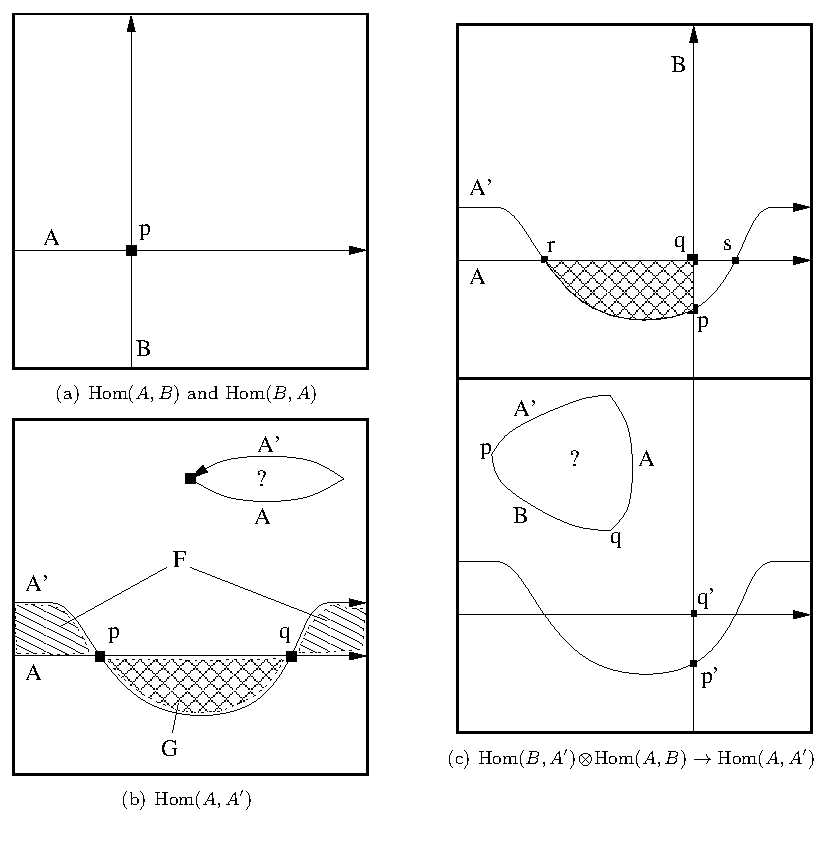
\includegraphics[width=0.95\linewidth]{figures/fig2.pdf}
  \caption{计算 Floer 链复形的图示：(a) $\mathrm{Hom}(A,B)$ 与 $\mathrm{Hom}(B,A)$；(b) $\mathrm{Hom}(A,A')$；(c) $\mathrm{Hom}(B,A')\otimes\mathrm{Hom}(A,B)\to\mathrm{Hom}(A,A')$。（原文 Figure 2，第 37 页）}
  \label{fig:floer-complex}
\end{figure}

接下来考虑 $\mathrm{Hom}(A,A)$。我们已由定理~\ref{thm:4.2} 知道它的上同调代数必同构于奇异上同调 $H^*(A,\Lambda_t)$，而后者是 $\Lambda_t\oplus\Lambda_t(-1)$（因为 $A$ 是圆周）。把 $A$ 作一个小的微扰、得到一条哈密顿同伦的曲线 $A'$ 来计算它，似乎更有启发性。这样的一个微扰如子图~\ref{fig:floer-complex}(b) 所示。我们看到 $\mathrm{Hom}(A,A')$ 是二维的，由 $p$ 与 $q$ 生成。又注意 $\tilde{s}_{A'}(p)=-\epsilon<0$，故 $\mu_p(A,A')=-[-\epsilon-0]=1$。相反地，$\tilde{s}_{A'}(q)=\epsilon>0$，故 $\mu_q(A,A')=0$。于是 $\mathrm{Hom}(A,A')$ 可能带有非零微分 $d(q)=\lambda p$。由第~\ref{subsec:fuk-surface} 小节对 Fukaya 范畴的描述，我们通过寻找以 $A$ 与 $A'$ 为边的浸入二边形（immersed bigon，模等价）来确定该微分。供参考，这类二边形的形状已画在图中。可以看出恰有两个这样的二边形，在图中标为 $F$ 与 $G$。于是
\[
dq=(t^F\pm t^G)p.
\]
这里的符号取决于我们尚未说明的约定。但注意必须有 $\mathrm{Hom}_{H\mathrm{Fuk}}(A,A')\neq0$，因为该集合中必有一个元素代表 $\mathbf{1}_A$。这只有在 $dq=0$ 时才能发生，而此时确实有 $\mathrm{Hom}_{H\mathrm{Fuk}}(A,A')\simeq H^*(A,\Lambda_t)$，与预期一致。还要注意 $dq=0$ 确实是可能的：微扰是哈密顿的，故 $F$ 与 $G$ 面积相同，于是若取上式的负号就有 $dq=0$。

% [Tutor Note: 易错点（Floer 微分符号与取向）：$dq=(t^F\pm t^G)p$ 的符号由曲线定向与圆盘的面积形式共同决定，原文未固定该约定。真正不依赖约定的是“$F$ 与 $G$ 面积相等”（微扰是哈密顿的，两条二边形面积相同），于是 $t^F=t^G$：取负号时两项相消得 $dq=0$；取正号则 $dq\ne0$，与 $\mathbf{1}_A\in\mathrm{Hom}_{H\mathrm{Fuk}}(A,A')$ 矛盾。换言之，$1_A$ 的存在性反过来定出了符号约定。]

对 $\mathrm{Hom}(B,B)$ 有类似的论证。于是我们发现，作为向量空间
\[
H(\mathcal{Q})\simeq Q
\]
（其中 $Q$ 仍是命题~\ref{prop:6.2} 中的代数）。与考察椭圆曲线的 Ext 代数时一样，几乎所有合成又都由形式理由确定；并且只要说明
\[
\mathrm{Hom}_{H\mathrm{Fuk}}(A,B)\,\mathrm{Hom}_{H\mathrm{Fuk}}(B,A)\neq0,
\qquad
\mathrm{Hom}_{H\mathrm{Fuk}}(B,A)\,\mathrm{Hom}_{H\mathrm{Fuk}}(A,B)\neq0,
\]
就能证明 $H(\mathcal{Q})\simeq Q$ 作为代数成立。也就是说，我们需要确定某个 $m_2$，即数一些三角形。现在考察子图~\ref{fig:floer-complex}(c)。我们将说明映射
\[
\mathrm{Hom}_{H\mathrm{Fuk}}(B,A')\otimes\mathrm{Hom}_{H\mathrm{Fuk}}(A,B)\longrightarrow
\mathrm{Hom}_{H\mathrm{Fuk}}(A,A')\simeq\mathrm{Hom}_{H\mathrm{Fuk}}(A,A)
\]
不是零映射。图中我们有两条经线 $A$ 与 $B$，以及 $A$ 的微扰 $A'$。为便于说明，我们画了表示环面的正方形的两份拷贝，把它们看作格 $\mathbb{Z}^2\subset\mathbb{R}^2$ 的两个基本域。在 $T$ 上，如前所述 $A$ 与 $B$ 有唯一交点，记为 $q$。点 $q'$ 与它等价。类似地，$A'$ 与 $B$ 交于唯一一点 $p$，图中还画出了另一个等价的交点 $p'$。又 $A'$ 与 $A$ 交于 $r$ 与 $s$。如前所述，我们确定 $|q|=0$、$|p|=1$、$|r|=1$、$|s|=0$。我们猜测
\[
m_2(p,q)=\lambda r,\qquad \lambda\neq0.
\]
（事实上，在 $B$ 与 $A'$ 的交点中，$r$ 是唯一具有正确次数的点。）正如第~\ref{subsec:fuk-surface} 小节所解释的，要计算这个乘积，需要数三角形。我们要找的三角形类型已画在图中：以 $q$、$p$ 和 $x$ 为顶点（按顺时针次序）、沿图中所示曲线段相连的三角形。图中我们还给一个这样的三角形画了阴影。

% [Tutor Note: 几何直观（多边形计数的面积权重）：$m_2$ 的三角形计数就是 Floer 复形中“两个交点合成第三个交点”的圆盘计数；在 $\Lambda_t$ 中每个圆盘以 $q^{\mathrm{area}}$ 加权（$q=e^{-t}$，面积越大权越小），因此只有面积相同的圆盘才会相消。这里 $y$ 坐标的单调性论证给出“唯一性”，避免了对全部格点平移求和的无穷计数——这正是环面的 Floer 同调能显式算出的根源。]

现在的主要观察是：在等价意义下这是唯一的这种三角形。也就是说，它是唯一以 $q$ 本身（而非某个等价点）为顶点的这种三角形。事实上，这种三角形的边 $q\to p$ 是 $y$ 坐标能改变超过 $1$ 的唯一一条边；即使沿另外两条边合起来，$y$ 坐标也绝不可能改变 $1$（因为另外两条边落在 $A$ 或 $A'$ 上）。但绕整个三角形一周必须使 $y$ 坐标不变，所以若它在某处改变超过 $1$，就必须改变两次，而这是不可能的。由此三角形的第二个顶点必须落在与我们出发时相同的基本域内，即它必须是 $p$。剩下的就简单了：三角形到 $T$ 的映射必须是保向的，且在角点之外是嵌入。于是三角形的第二条边必须“向左出发”（由定向决定），而第三个顶点必须是 $r$（而不是它的某个平移），否则我们无法得到嵌入。

另一个合成的处理与之完全相同，于是抽象镜像对称的证明到此完成。

% [Tutor Note: 记号提示：图~\ref{fig:floer-complex}(c) 中以“?”标出的那个顶点，正是正文所记的三角形第三个顶点 $x$；论证的结论是它必须等于 $r$（而不是 $r$ 的某个平移），故正文结尾说“第三个顶点必须是 $r$”。又，图 (c) 下半部分标出的 $q'$、$p'$ 是 $q$、$p$ 在相邻基本域中的等价点，对照画出的两份正方形即可看出平移关系。]
